\noindent\textbf{Goal:} take the already known matrix columns, reconstruct each
row, and attach an identity row. This step does not invert anything yet. The
result is the starting augmented matrix for the next step.

\begin{Verbatim}
rows = []
for row_index in range(32):
    matrix_row = 0
    for column_index in range(32):
        output_bit = (columns[column_index] >> row_index) & 1
        matrix_row |= output_bit << column_index
    identity_bit = 1 << (32 + row_index)
    augmented_row = matrix_row | identity_bit
    rows.append(augmented_row)
\end{Verbatim}
\noindent Indentation is essential: the identity is attached \emph{after} all
columns of one row have been read. The function appends one packed integer per
outer-loop iteration, not one integer per cell.

\subsubsection*{A drawing at the exact point where the bit is read}
Use a four-bit teaching matrix, with stored columns
$[\texttt{0101},\texttt{0011},\texttt{0010},\texttt{1000}]$ in binary.
The highlighted cell is row 1, column 1. Matrix rows run downward; matrix
columns run rightward. Printed binary numbers put bit 0 on the right.

\begin{center}
\begin{tikzpicture}[x=8mm,y=8mm,every node/.style={font=\small}]
\foreach \r/\a/\b/\c/\d in {0/1/1/0/0,1/0/1/1/0,2/1/0/0/0,3/0/0/0/1}{
\foreach \j/\v in {0/\a,1/\b,2/\c,3/\d}{
\def\shade{white}\ifnum\j=1\def\shade{blue!12}\fi
\ifnum\r=1\def\shade{teal!15}\fi
\ifnum\r=1\ifnum\j=1\def\shade{orange!30}\fi\fi
\node[draw,fill=\shade,minimum size=8mm] at (\j,-\r) {\v};}
\node[left] at (-.6,-\r) {$r=\r$};}
\foreach \j in {0,1,2,3}{\node at (\j,.85) {\j};}
\node at (1.5,1.5) {column $c$};
\foreach \r/\v in {0/1,1/1,2/0,3/0}{
\def\shade{blue!12}\ifnum\r=1\def\shade{orange!30}\fi
\node[draw,fill=\shade,minimum size=8mm] at (6,-\r) {\v};}
\node[align=center] at (6,1.1) {\hx{columns[1]}};
\draw[-{Stealth},thick,blue!65!black] (3.6,-1)--(5.4,-1);
\node[align=center] at (6,-4) {top to bottom: $[1,1,0,0]$\\stored integer: \hx{0011}};
\node[draw,fill=orange!30,align=center] (out) at (11,-1) {\hx{output\_bit = 1}};
\draw[-{Stealth},thick,orange!80!black] (6.6,-1)--node[above] {\hx{>> 1}, then \hx{\& 1}} (out.west);
\node[align=center] at (11,-3) {Write at bit 1:\\$1\ll1=\texttt{0010}$};
\draw[-{Stealth},thick,teal!70!black] (out.south)--(11,-2.3);
\end{tikzpicture}
\end{center}
The column is not moved. We read one coefficient from its packed integer and
write that coefficient into the packed row being constructed.

\subsubsection*{Every line: substituted values, result, and purpose}
For the small example only, use width 4 instead of 32 in the two ranges and in
the identity shift. The next worked iteration has $r=1$, $c=1$.
The preceding column $c=0$ contributed 0, so the accumulated row is still
\hx{0000}. Binary words below are padded to four or eight positions; loop
indices and shift counts are decimal.

\paragraph{1. \texttt{rows = []}.}
Create an empty list of augmented rows. It will eventually contain four
integers in this example, or 32 in SM4. The list is initialized once, before
either loop. It must retain earlier rows when a new row begins.

\paragraph{2. \texttt{for row\_index in range(4):}.}
The outer iterator produces $0,1,2,3$. We are showing its second iteration,
so \hx{row\_index = 1}. This selects the matrix row to reconstruct; it stays
fixed throughout the inner loop. Row 0 has already been appended.

\paragraph{3. \texttt{matrix\_row = 0}.}
At the beginning of row 1, set the accumulator to \hx{0000}. This removes the
bits used to construct the previous row; reusing that row would mix unrelated
coefficients. This line executes once per row, not once per column.

\paragraph{4. \texttt{for column\_index in range(4):}.}
Visit $c=0,1,2,3$ within fixed row $r=1$. At $c=1$, read the second stored
column: \hx{columns[1] = 0011}. The position in the list selects a column;
the row index selects a bit within that column.

\paragraph{5. \texttt{output\_bit = (columns[column\_index] >> row\_index) \& 1}.}
Substitute each operand:
\[
\begin{aligned}
\hx{output\_bit}&=(\texttt{0011}\gg1)\mathbin{\&}\texttt{0001}\\
&=\texttt{0001}\mathbin{\&}\texttt{0001}=1.
\end{aligned}
\]
Why shift? To bring the coefficient for row 1 into bit position 0.
Why AND with 1? To discard all other coefficients and obtain exactly 0 or 1.
For contrast, column 0 gives
$(\texttt{0101}\gg1)\mathbin{\&}\texttt{0001}
=\texttt{0010}\mathbin{\&}\texttt{0001}=0$.
The extra 1 in position 1 is irrelevant to this selected matrix entry.

\paragraph{6. \texttt{matrix\_row |= output\_bit << column\_index}.}
The augmented assignment is shorthand for
\hx{matrix\_row = matrix\_row | (output\_bit << column\_index)}.
For $c=1$ the complete update is
\[
\hx{matrix\_row}=\texttt{0000}\,|\,(1\ll1)
=\texttt{0000}\,|\,\texttt{0010}=\texttt{0010}.
\]
Why shift left? In the reconstructed row, column $c$ is stored at bit position
$c$. Why OR? Set that position while preserving all previously assembled bits.
In the next iteration $c=2$, another extracted 1 contributes \hx{0100}:
\[
\texttt{0010}\,|\,(1\ll2)
=\texttt{0010}\,|\,\texttt{0100}=\texttt{0110}.
\]
Column 3 contributes 0, so the completed row remains \hx{0110}.

\paragraph{7. \texttt{identity\_bit = 1 << (4 + row\_index)}.}
This line executes after the inner loop. Use $r=1$:
\[
\hx{identity\_bit}=1\ll(4+1)=1\ll5=\texttt{00100000}.
\]
Why add 4? The low four positions already hold the matrix row. The identity
must occupy the next four positions. Why add $r$? Row $r$ of the identity has
its 1 in column $r$. In SM4 this expression uses $32+r$, not $4+r$.

\paragraph{8. \texttt{augmented\_row = matrix\_row | identity\_bit}.}
Pad both operands to eight bits before combining them:
\[
\begin{array}{rcl}
\text{matrix row}&=&\texttt{0000\ 0110}\\
\text{identity row}&=&\texttt{0010\ 0000}\\\hline
\text{bitwise OR}&=&\texttt{0010\ 0110}.
\end{array}
\]
The result is decimal 38, hexadecimal \hx{26}. OR does not mean concatenating
decimal numbers: the two integers occupy non-overlapping bit positions.

\begin{center}
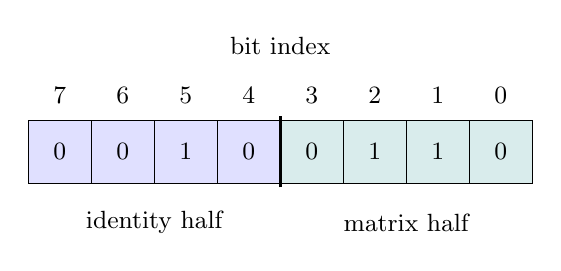
\begin{tikzpicture}[x=8mm,y=9mm,every node/.style={font=\small}]
\foreach \j/\b/\v in {0/7/0,1/6/0,2/5/1,3/4/0,4/3/0,5/2/1,6/1/1,7/0/0}{
\def\shade{blue!12}\ifnum\j>3\def\shade{teal!15}\fi
\node[draw,fill=\shade,minimum size=8mm] at (\j,0) {\v};
\node at (\j,.8) {\b};}
\node at (3.5,1.5) {bit index};
\draw[very thick] (3.5,-.5)--(3.5,.5);
\node at (1.5,-1) {identity half};\node at (5.5,-1) {matrix half};
\end{tikzpicture}
\end{center}
Mathematics writes $[M\mid I]$, but a printed integer lists its high half first,
so storage appears as $[I\mid M]$. The row operations will act on both halves.

\paragraph{9. \texttt{rows.append(augmented\_row)}.}
Row 0 previously produced \hx{00010011} (hex \hx{13}). Append row 1's
\hx{00100110} (hex \hx{26}):
\[
\hx{rows}=[\hx{13}]\quad\longrightarrow\quad[\hx{13},\hx{26}]
\qquad\text{(hexadecimal entries)}.
\]
Then the outer loop advances to row 2, resets the accumulator, and repeats.
This append is why completed rows are not lost when \hx{matrix\_row} is reset.

\subsubsection*{The complete four-bit run: every iteration, no guessed values}
In each table, $C$ is the stored column; ``shifted'' is $C\gg r$;
$b=(C\gg r)\mathbin{\&}1$; ``placed'' is $b\ll c$; and ``row before/after''
shows the OR accumulator. Padded digit strings are binary; the row and column
indices, shift counts and decimal shift results are ordinary decimal integers.
\paragraph{Outer iteration: row\_index = 0.}
Start with \hx{matrix\_row = 0000}.
\begin{center}\small\begin{tabular}{rllllll}\toprule
$c$ & $C$ & Shifted & $b$ & Placed & Row before & Row after\\\midrule
0 & 0101 & 0101 & 1 & 0001 & 0000 & 0001\\
1 & 0011 & 0011 & 1 & 0010 & 0001 & 0011\\
2 & 0010 & 0010 & 0 & 0000 & 0011 & 0011\\
3 & 1000 & 1000 & 0 & 0000 & 0011 & 0011\\
\bottomrule\end{tabular}\end{center}
\[\begin{aligned}
\hx{identity\_bit}&=1\ll(4+0)=16=\hx{00010000},\\
\hx{augmented\_row}&=\hx{00000011}\,|\,\hx{00010000}=\hx{00010011}.\end{aligned}\]
Append to \hx{rows}. List so far (hex): \hx{13}.
\paragraph{Outer iteration: row\_index = 1.}
Start with \hx{matrix\_row = 0000}.
\begin{center}\small\begin{tabular}{rllllll}\toprule
$c$ & $C$ & Shifted & $b$ & Placed & Row before & Row after\\\midrule
0 & 0101 & 0010 & 0 & 0000 & 0000 & 0000\\
1 & 0011 & 0001 & 1 & 0010 & 0000 & 0010\\
2 & 0010 & 0001 & 1 & 0100 & 0010 & 0110\\
3 & 1000 & 0100 & 0 & 0000 & 0110 & 0110\\
\bottomrule\end{tabular}\end{center}
\[\begin{aligned}
\hx{identity\_bit}&=1\ll(4+1)=32=\hx{00100000},\\
\hx{augmented\_row}&=\hx{00000110}\,|\,\hx{00100000}=\hx{00100110}.\end{aligned}\]
Append to \hx{rows}. List so far (hex): \hx{13, 26}.
\paragraph{Outer iteration: row\_index = 2.}
Start with \hx{matrix\_row = 0000}.
\begin{center}\small\begin{tabular}{rllllll}\toprule
$c$ & $C$ & Shifted & $b$ & Placed & Row before & Row after\\\midrule
0 & 0101 & 0001 & 1 & 0001 & 0000 & 0001\\
1 & 0011 & 0000 & 0 & 0000 & 0001 & 0001\\
2 & 0010 & 0000 & 0 & 0000 & 0001 & 0001\\
3 & 1000 & 0010 & 0 & 0000 & 0001 & 0001\\
\bottomrule\end{tabular}\end{center}
\[\begin{aligned}
\hx{identity\_bit}&=1\ll(4+2)=64=\hx{01000000},\\
\hx{augmented\_row}&=\hx{00000001}\,|\,\hx{01000000}=\hx{01000001}.\end{aligned}\]
Append to \hx{rows}. List so far (hex): \hx{13, 26, 41}.
\paragraph{Outer iteration: row\_index = 3.}
Start with \hx{matrix\_row = 0000}.
\begin{center}\small\begin{tabular}{rllllll}\toprule
$c$ & $C$ & Shifted & $b$ & Placed & Row before & Row after\\\midrule
0 & 0101 & 0000 & 0 & 0000 & 0000 & 0000\\
1 & 0011 & 0000 & 0 & 0000 & 0000 & 0000\\
2 & 0010 & 0000 & 0 & 0000 & 0000 & 0000\\
3 & 1000 & 0001 & 1 & 1000 & 0000 & 1000\\
\bottomrule\end{tabular}\end{center}
\[\begin{aligned}
\hx{identity\_bit}&=1\ll(4+3)=128=\hx{10000000},\\
\hx{augmented\_row}&=\hx{00001000}\,|\,\hx{10000000}=\hx{10001000}.\end{aligned}\]
Append to \hx{rows}. List so far (hex): \hx{13, 26, 41, 88}.


The loop terminates with four packed rows. Only now does Gaussian elimination
begin. No ciphertext, plaintext or secret key was needed to construct these
public matrix rows.

\subsubsection*{Back to real SM4: the exact same statements with width 32}
For \hx{row\_index = 1} and \hx{column\_index = 1}, the real column is
$L(2^1)=\hx{0208080A}$. The previous column gave a zero coefficient in this row,
so \hx{matrix\_row = 0}. Substitute the real values:
\[
\begin{aligned}
\hx{output\_bit}&=(\hx{0208080A}\gg1)\mathbin{\&}1\\
&=\hx{01040405}\mathbin{\&}1=1,\\
\hx{matrix\_row}&=\hx{00000000}\,|\,(1\ll1)=\hx{00000002}.
\end{aligned}
\]
The following table completes this real row across all 32 columns. Hexadecimal
is used for 32-bit words to avoid wrapping long binary strings; $b$ is a single
bit. Every cell extraction and accumulation is included for this one row.
\begingroup\small\begin{longtable}{rllrlll}\toprule
$c$ & $L(2^c)$ & Shifted by 1 & $b$ & Placed & Row before & Row after\\\midrule
\endhead
0 & 01040405 & 00820202 & 0 & 00000000 & 00000000 & 00000000\\
1 & 0208080A & 01040405 & 1 & 00000002 & 00000000 & 00000002\\
2 & 04101014 & 0208080A & 0 & 00000000 & 00000002 & 00000002\\
3 & 08202028 & 04101014 & 0 & 00000000 & 00000002 & 00000002\\
4 & 10404050 & 08202028 & 0 & 00000000 & 00000002 & 00000002\\
5 & 208080A0 & 10404050 & 0 & 00000000 & 00000002 & 00000002\\
6 & 41010140 & 208080A0 & 0 & 00000000 & 00000002 & 00000002\\
7 & 82020280 & 41010140 & 0 & 00000000 & 00000002 & 00000002\\
8 & 04040501 & 02020280 & 0 & 00000000 & 00000002 & 00000002\\
9 & 08080A02 & 04040501 & 1 & 00000200 & 00000002 & 00000202\\
10 & 10101404 & 08080A02 & 0 & 00000000 & 00000202 & 00000202\\
11 & 20202808 & 10101404 & 0 & 00000000 & 00000202 & 00000202\\
12 & 40405010 & 20202808 & 0 & 00000000 & 00000202 & 00000202\\
13 & 8080A020 & 40405010 & 0 & 00000000 & 00000202 & 00000202\\
14 & 01014041 & 0080A020 & 0 & 00000000 & 00000202 & 00000202\\
15 & 02028082 & 01014041 & 1 & 00008000 & 00000202 & 00008202\\
16 & 04050104 & 02028082 & 0 & 00000000 & 00008202 & 00008202\\
17 & 080A0208 & 04050104 & 0 & 00000000 & 00008202 & 00008202\\
18 & 10140410 & 080A0208 & 0 & 00000000 & 00008202 & 00008202\\
19 & 20280820 & 10140410 & 0 & 00000000 & 00008202 & 00008202\\
20 & 40501040 & 20280820 & 0 & 00000000 & 00008202 & 00008202\\
21 & 80A02080 & 40501040 & 0 & 00000000 & 00008202 & 00008202\\
22 & 01404101 & 00A02080 & 0 & 00000000 & 00008202 & 00008202\\
23 & 02808202 & 01404101 & 1 & 00800000 & 00008202 & 00808202\\
24 & 05010404 & 02808202 & 0 & 00000000 & 00808202 & 00808202\\
25 & 0A020808 & 05010404 & 0 & 00000000 & 00808202 & 00808202\\
26 & 14041010 & 0A020808 & 0 & 00000000 & 00808202 & 00808202\\
27 & 28082020 & 14041010 & 0 & 00000000 & 00808202 & 00808202\\
28 & 50104040 & 28082020 & 0 & 00000000 & 00808202 & 00808202\\
29 & A0208080 & 50104040 & 0 & 00000000 & 00808202 & 00808202\\
30 & 40410101 & 20208080 & 0 & 00000000 & 00808202 & 00808202\\
31 & 80820202 & 40410101 & 1 & 80000000 & 00808202 & 80808202\\
\bottomrule\end{longtable}\endgroup

After the last column, the result is \hx{80808202}. Its set positions are
1, 9, 15, 23 and 31. These are row coefficients, not the set positions in a
single column $L(2^c)$; rotations wrap around the word. Attach the identity:
\[
\begin{aligned}
\hx{identity\_bit}&=1\ll(32+1)=\hx{0000000200000000},\\
\hx{augmented\_row}&=\hx{0000000080808202}\,|\,\hx{0000000200000000}\\
&=\boxed{\hx{0000000280808202}}.
\end{aligned}
\]
The high 32 bits are \hx{00000002}, identity row 1; the low 32 bits are
\hx{80808202}, matrix row 1. This is a complete SM4 row, ready to append to
\hx{rows}. The other rows use their own row indices but exactly the same rule.
